\documentclass[12pt,letterpaper]{article}
\usepackage[utf8]{inputenc}
\usepackage{amsmath}
\usepackage{amsfonts}
\usepackage{amssymb}
\usepackage{graphicx}
\usepackage[left=0.79in, right=0.79in, top=0.79in, bottom=0.79in]{geometry}
\author{Chathan Driehuys}

\graphicspath{{./images/}}

\begin{document}
	\section*{Task 1}
		In order to exploit the \texttt{stack.c} program, the first step was to figure out where the return address that we needed to override was. Using \texttt{gdb} we could easily obtain this address after setting a breakpoint in the \texttt{bof} function.
		
		To compute the return address' offset from the buffer we were overflowing, we had to determine the structure of the stack. After some digging we discovered that before the return address was the 4 byte frame pointer and prior to that was the buffer padded out to 32 bytes.
		
		After calculating the offset of the return address from the buffer, we inserted a new address pointing to (or slightly before) the provided shellcode.
	
	\section*{Task 2}
		When enabling address space randomization, it becomes more difficult to insert the return address in the correct position since we don't know its offset from the buffer that we are overflowing. With no changes to the exploit program created in Task 1 we can brute force the randomization until it matches the addresses we encountered in the first exercise.
	
		\begin{figure}[h]
			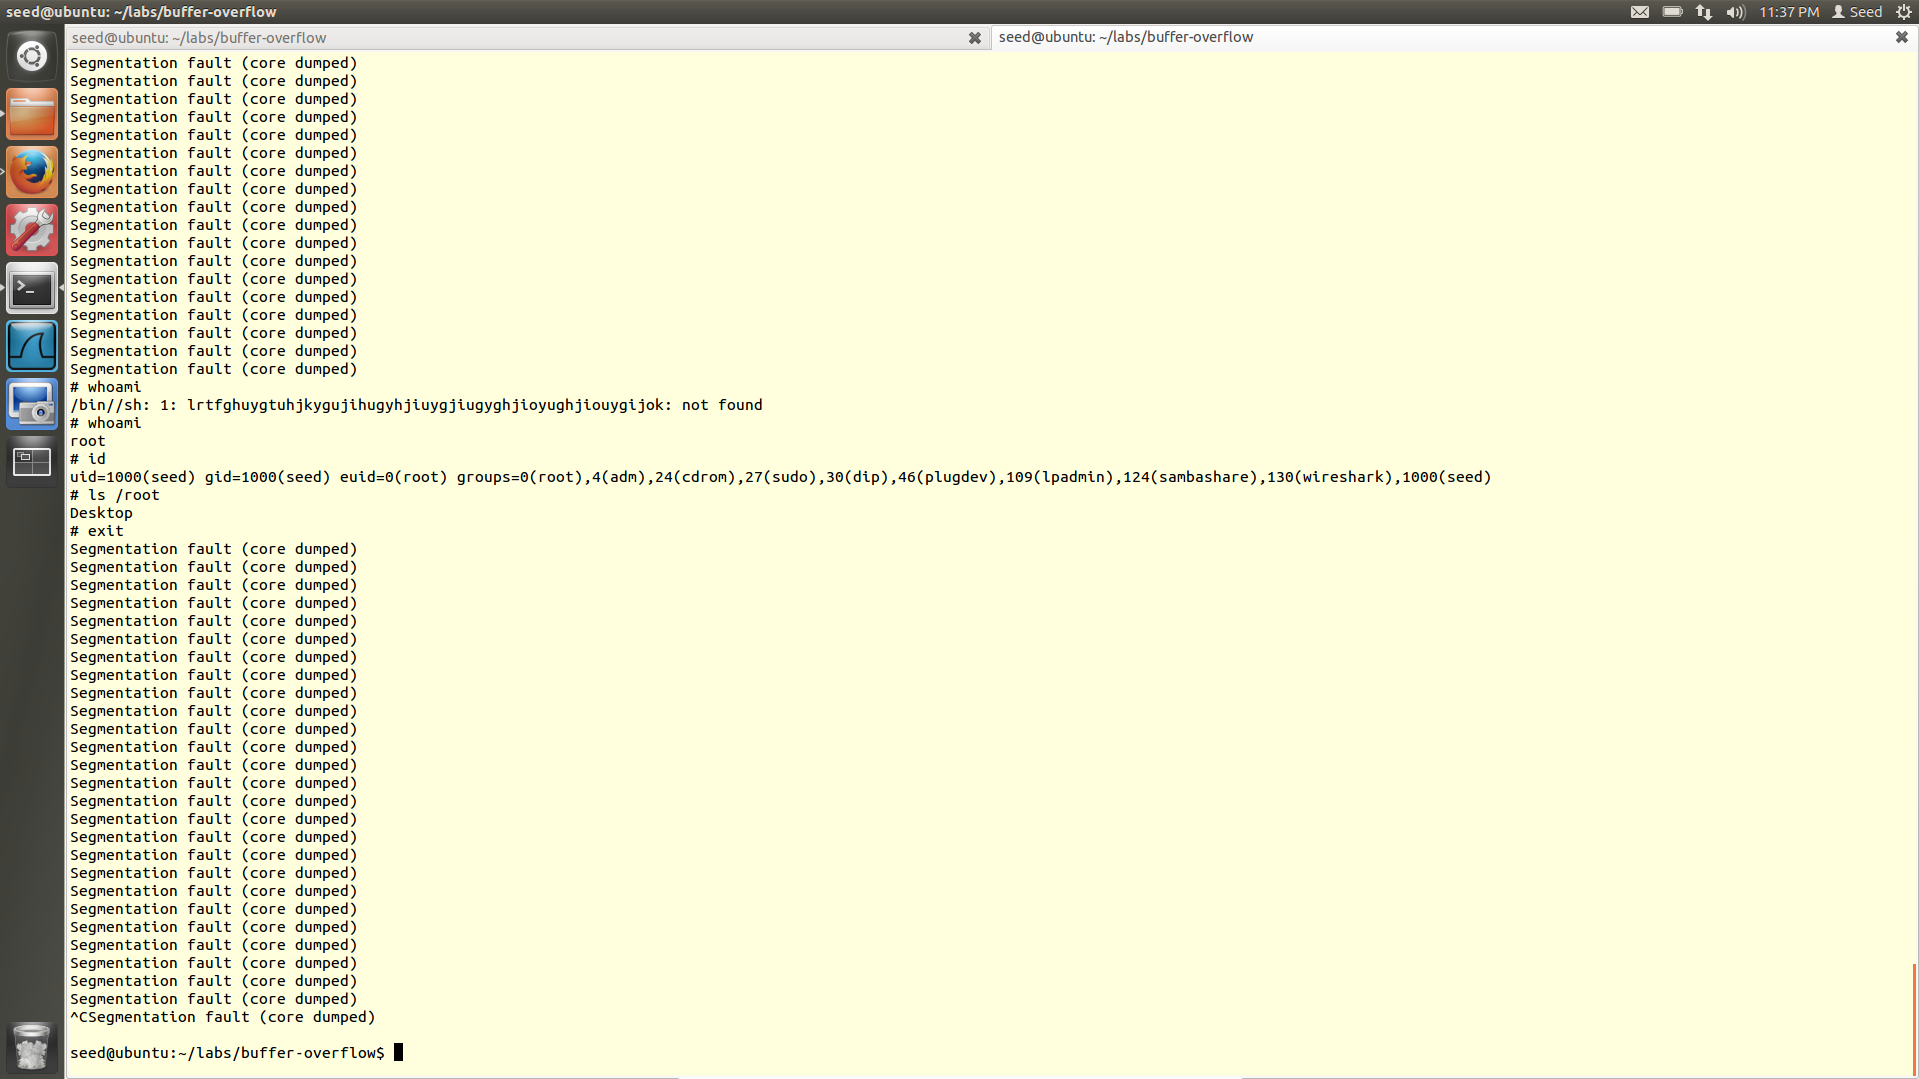
\includegraphics[width=\linewidth]{task-2}
			\caption{Eventually getting a root shell with address randomization enabled.}
		\end{figure}
		
		The figure above is the result of roughly two hours of running our original exploit until the addresses worked out. In order to optimize the process we could fill the beginning of the buffer with our intended return address to maximize the chances that we put it in the correct place.
		
	\section*{Task 3}
		If we attempt to perform Task 1 without disabling the ``Stack Guard'', we receive an error about ``stack smashing''.
		
		\begin{verbatim}
			seed@ubuntu:~/labs/buffer-overflow$ ./stack 
			*** stack smashing detected ***: ./stack terminated
			Segmentation fault (core dumped)
		\end{verbatim}
		
		A cursory search for stack smashing indicates that \texttt{gcc} provides a buffer overflow protection that inserts canary values after buffers that can then be checked to determine if they have been overflowed.\footnote{https://stackoverflow.com/questions/1345670/stack-smashing-detected}
		
	\section*{Task 4}
		If we prevent the stack from being executable, our exploit no longer works. The buffer overflow still works but the instructions we inserted cannot be executed because they are contained in the stack.
		
		\begin{verbatim}
			seed@ubuntu:~/labs/buffer-overflow$ ./stack 
			Segmentation fault (core dumped)
		\end{verbatim}
\end{document}